\documentclass[tikz,border=12pt]{standalone}
\usepackage[T1]{fontenc}
\usepackage{mathpazo}
\usepackage{amsmath,amssymb}
\usetikzlibrary{arrows.meta, positioning, calc, fit, patterns, decorations.pathreplacing}

\definecolor{stblue}{HTML}{7B97AD}
\definecolor{rwgold}{HTML}{B8995E}
\definecolor{sage}{HTML}{7A9A7E}
\definecolor{dkbrown}{HTML}{3D3530}
\definecolor{wmgray}{HTML}{7B7067}
\definecolor{cream}{HTML}{F9F6F0}
\definecolor{border}{HTML}{D4C9B8}
\definecolor{terracotta}{HTML}{C47A6A}
\definecolor{lavender}{HTML}{907EA0}

\begin{document}
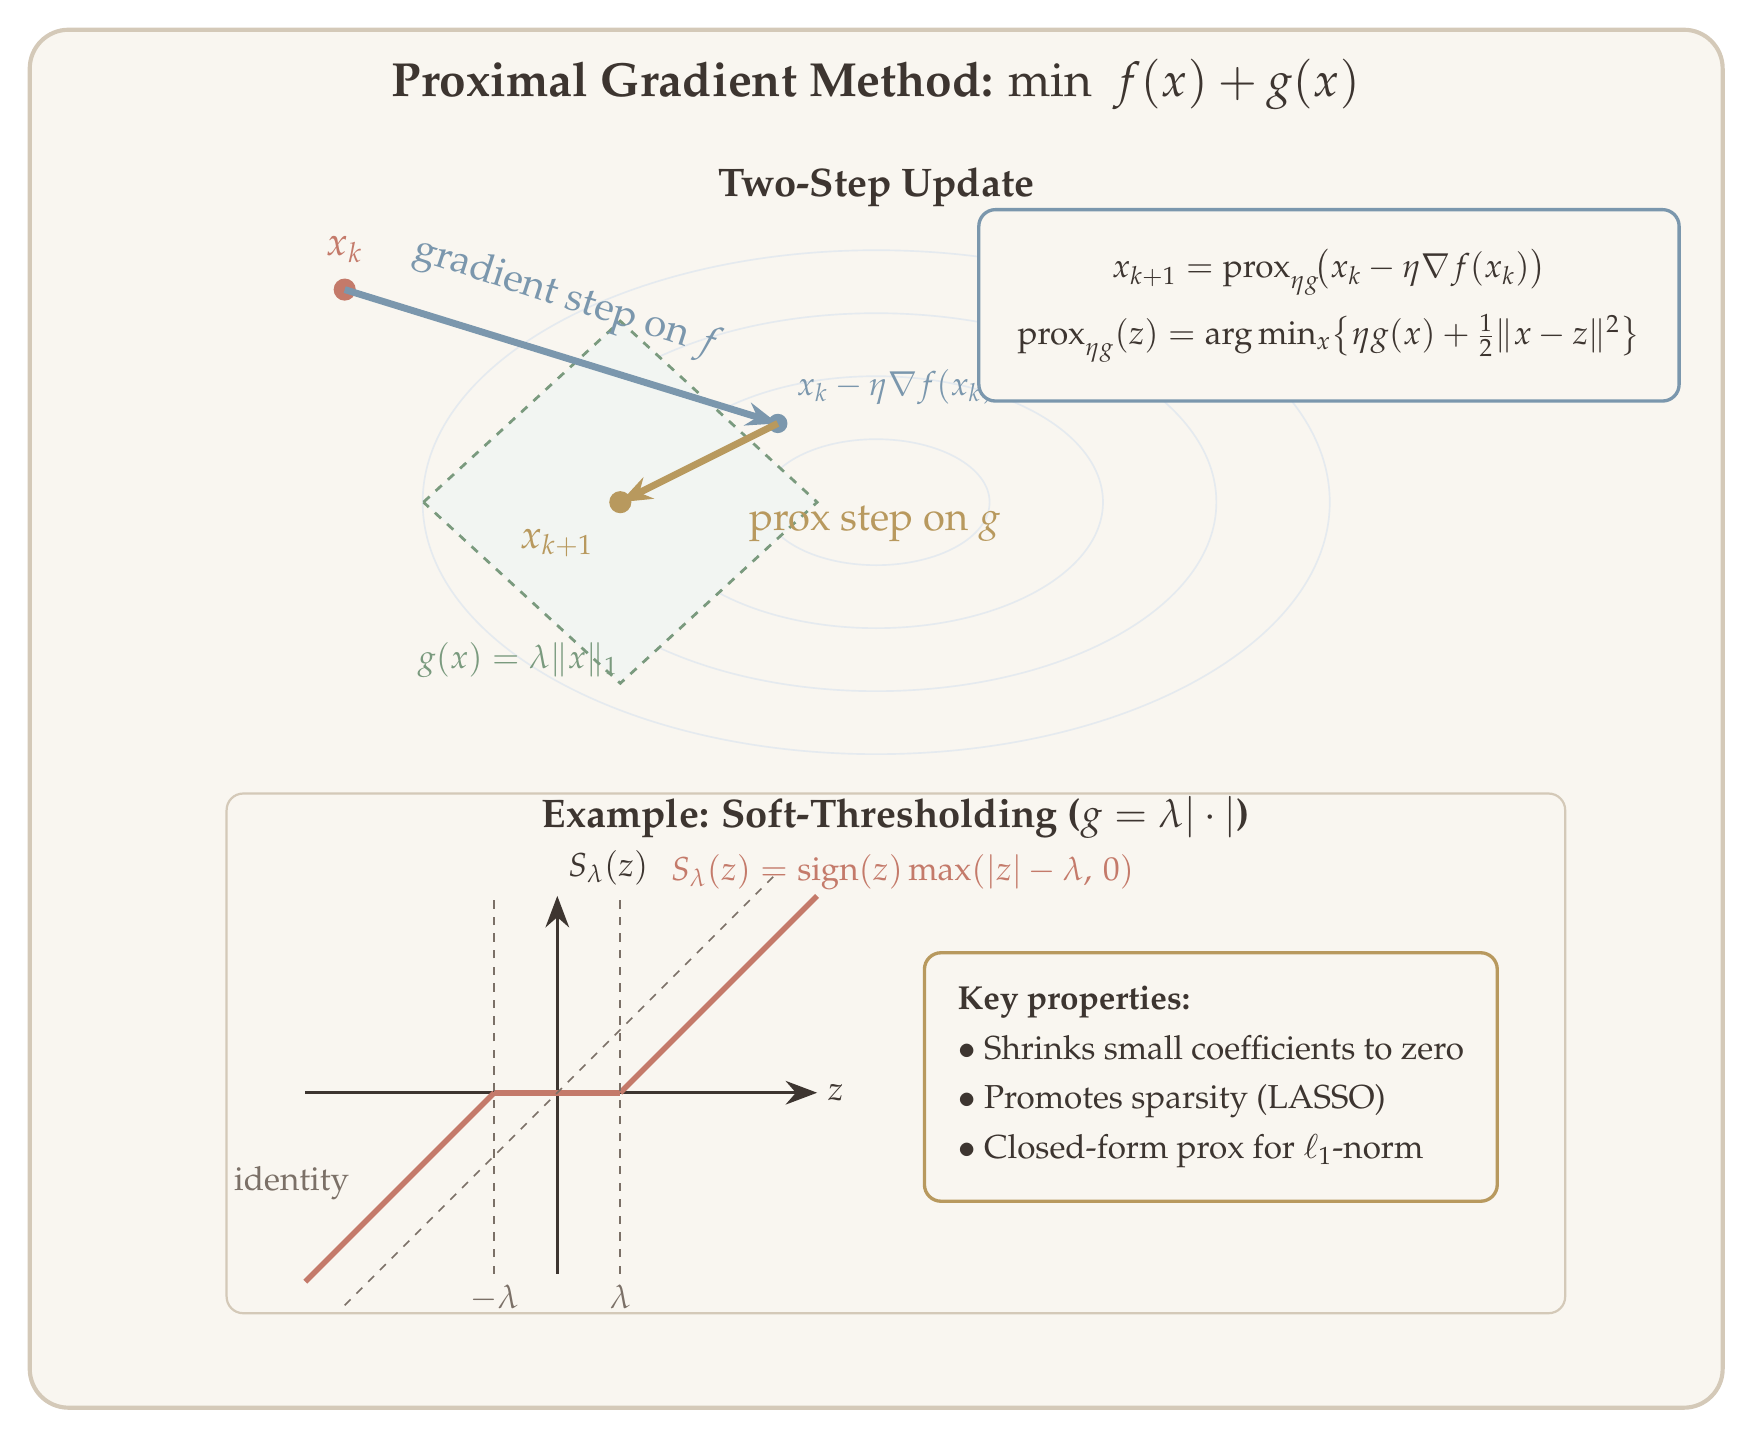
\begin{tikzpicture}[>={Stealth[length=4mm, width=3mm]}, line width=1.5pt]

% Background
\fill[cream, rounded corners=14pt] (-2,-8) rectangle (19.5,9.5);
\draw[border, line width=1.5pt, rounded corners=14pt] (-2,-8) rectangle (19.5,9.5);

% Title
\node[font=\LARGE\bfseries, text=dkbrown] at (8.75,8.8) {Proximal Gradient Method: $\min\; f(x) + g(x)$};

% =========== TOP: Proximal gradient step diagram ===========
\node[font=\Large\bfseries, text=dkbrown] at (8.75,7.5) {Two-Step Update};

% Contour lines background (elliptical for f)
\foreach \r in {0.8, 1.6, 2.4, 3.2} {
  \draw[stblue!20, line width=0.6pt] (8.75,3.5) ellipse ({1.8*\r} and {\r});
}

% Constraint / regularization region (L1 ball - diamond shape)
\fill[sage!10] (3,3.5) -- (5.5,5.8) -- (8,3.5) -- (5.5,1.2) -- cycle;
\draw[sage, line width=1pt, dashed] (3,3.5) -- (5.5,5.8) -- (8,3.5) -- (5.5,1.2) -- cycle;
\node[font=\large, text=sage] at (4.2,1.5) {$g(x) = \lambda\|x\|_1$};

% Point x_k
\fill[terracotta] (2,6.2) circle (4pt);
\node[font=\Large, text=terracotta, above] at (2,6.4) {$x_k$};

% Gradient step arrow (long)
\draw[->, stblue, line width=2.5pt] (2,6.2) -- (7.5,4.5);
\node[font=\Large, text=stblue, above, rotate=-18] at (4.7,5.7) {gradient step on $f$};

% Intermediate point
\fill[stblue] (7.5,4.5) circle (3.5pt);
\node[font=\large, text=stblue, above right] at (7.6,4.6) {$x_k - \eta\nabla f(x_k)$};

% Prox step arrow
\draw[->, rwgold, line width=2.5pt] (7.5,4.5) -- (5.5,3.5);
\node[font=\Large, text=rwgold, below right] at (7.0,3.6) {prox step on $g$};

% Final point x_{k+1}
\fill[rwgold] (5.5,3.5) circle (4pt);
\node[font=\Large, text=rwgold, below left] at (5.3,3.3) {$x_{k+1}$};

% Formula box
\node[fill=cream, draw=stblue, line width=1.2pt, rounded corners=6pt,
      font=\large, text=dkbrown, align=center, inner sep=14pt]
  at (14.5,6.0) {$x_{k+1} = \mathrm{prox}_{\eta g}\!\bigl(x_k - \eta\nabla f(x_k)\bigr)$\\[6pt]
  $\mathrm{prox}_{\eta g}(z) = \arg\min_x \bigl\{\eta g(x) + \tfrac{1}{2}\|x-z\|^2\bigr\}$};

% =========== BOTTOM: Soft-thresholding ===========
\draw[border, line width=0.8pt, rounded corners=6pt] (0.5,-6.8) rectangle (17.5,-0.2);
\node[font=\Large\bfseries, text=dkbrown] at (9,-0.5) {Example: Soft-Thresholding ($g = \lambda|\cdot|$)};

% Axes for soft-thresholding
\draw[->, dkbrown, line width=1.2pt] (1.5,-4.0) -- (8,-4.0) node[right, font=\large, text=dkbrown] {$z$};
\draw[->, dkbrown, line width=1.2pt] (4.7,-6.3) -- (4.7,-1.5) node[above right, font=\large, text=dkbrown] {$S_\lambda(z)$};

% Soft thresholding function
% Left branch
\draw[terracotta, line width=2pt, domain=1.5:3.9]
  plot (\x, {(\x - 4.7) + 0.8 - 4.0});
% Flat part
\draw[terracotta, line width=2pt] (3.9,-4.0) -- (5.5,-4.0);
% Right branch
\draw[terracotta, line width=2pt, domain=5.5:8]
  plot (\x, {(\x - 4.7) - 0.8 - 4.0});

% Lambda markers
\draw[wmgray, dashed, line width=0.6pt] (3.9,-6.3) -- (3.9,-1.5);
\draw[wmgray, dashed, line width=0.6pt] (5.5,-6.3) -- (5.5,-1.5);
\node[font=\large, text=wmgray, below] at (3.9,-6.3) {$-\lambda$};
\node[font=\large, text=wmgray, below] at (5.5,-6.3) {$\lambda$};

% Identity line for reference
\draw[wmgray, line width=0.6pt, dashed, domain=2:7.5]
  plot (\x, {\x - 4.7 - 4.0});
\node[font=\large, text=wmgray, above left] at (2.2,-5.5) {identity};

% Formula
\node[font=\large, text=terracotta, anchor=west] at (6.0,-1.2) {$S_\lambda(z) = \mathrm{sign}(z)\max(|z|-\lambda,\, 0)$};

% Right side: interpretation
\node[fill=cream, draw=rwgold, line width=1.2pt, rounded corners=6pt,
      font=\large, text=dkbrown, align=left, inner sep=12pt]
  at (13,-3.8) {%
  \textbf{Key properties:}\\[4pt]
  $\bullet$ Shrinks small coefficients to zero\\[4pt]
  $\bullet$ Promotes sparsity (LASSO)\\[4pt]
  $\bullet$ Closed-form prox for $\ell_1$-norm};

\end{tikzpicture}
\end{document}
